\newpage
\section[Partielle Differentialgleichungen]{Partielle Differentialgleichungen}
\textit{Eine partielle Differentialgleichung ist eine Differentialgleichung, die partielle Ableitungen enthält. Sie gibt als Lösung also eine Funktion, die von mehreren Variablen abhängt. Ein sehr prominentes Beispiel ist die Schrödingengleichung:
$$i\hbar\frac{\partial}{\partial t}\Psi(\vec{x},t)=-\frac{\hbar^2}{2m}\triangle \Psi(\vec{x},t)+V(\vec{x})\Psi(\vec{x},t)$$
Wir starten mit partiellen Differentialgleichungen zweiter Ordnung. \\ \\
Dieses Thema lernt man, ähnlich wie für gewöhnliche DGLs, am besten an Beispielen.}
\begin{Def}{Partielle Differentialgleichungen zweiter Ordnung}
Wir suschen eine Funktion
$$U:G\rightarrow \R \quad (G\subseteq \R^n)$$
Für die Ableitungen schreiben wir abkürzend:
$$U_{x_j}=\frac{\partial u}{\partial x_j}\quad u_{x_jx_k}=\frac{\partial^2 u}{\partial x_j \partial x_k}$$
Die Funktion $u$ soll die partielle Differentialgleichung zweiter Ordnung
$$F(\underbrace{x_1,...,x_n}_n,\underbrace{u, u_{x_1},...,u_{x_n}}_{n+1}, \underbrace{u_{x_1x_1}, u_{x_1x_2},...,u_{x_nx_n}}_{n^2})=0$$
erfüllen. Hierbei ist $F$ eine Funktion
$$F: U\rightarrow \C \quad U\subseteq \R^{2n+1+n^2}$$
$U$ und $G$ müssen offen und wegzusammenhängend sein. Zusätzlich muss man noch eine Bedingung beachten:
\begin{enumerate}
    \item $(x_1,...,x_n, u(x), u_{x_1}(x),...,u_{x_n}(x), u_{x_1x_1}(x),...u_{x_n,x_n}(x))\in U \quad \forall x\in G$
    \item $F(x_1,...,x_n, u(x), u_{x_1}(x),...,u_{x_n}(x), u_{x_1x_1}(x),...u_{x_n,x_n}(x))=0 \quad \forall x\in G$
\end{enumerate}
\end{Def}
\begin{Def}{Speziallfall partieller Differentialgleichungen zweiter Ordnung}
Sei
$$A(u)+h=0 \qquad A(u)=\sum_{j,k=1}^n a_{jk}u_{x_j,x_k}$$
Man unterteilt Differentialgleichungen dieser Form in:
\begin{enumerate}
    \item \red{Quasilinear}: $a_{jk}$ und $h$ sind Funktionen von $x_1,...,x_n, u, u_{x_1},...,u_{x_n}$
    \item \red{Semilinear} oder \red{postlinear}: $a_{jk}$ ist eine Funktion von $x_1,...,x_n$ und $h$ von $x_1,...,x_n, u, u_{x_1},...,u_{x_n}$
    \item \red{Linear}: $h$ ist von der Form:
    $$h=\sum_{j=1}^n a_ju_{x_j}+au+f$$
    und $a_{jk}, a_j, a$ und $f$ sind Funktionen von $x_1, ..., x_n$.
    \item \red{Linear mit konstanten Koeffizienten}: Wie 3. nur sind $a_{jk}, a_j, a$ und $f$ konstant.
\end{enumerate}
\end{Def}
Die letzte Variante ist natürlich besonders benutzerfreundlich.
\subsection{Typen linearer PDGLs}
\begin{Def}{Typen von PDGLs mit konstanten Koeffizienten}
Man kann jede PDGL 2. Ordnung in die Form $$(\sum_{i,j} a_{ij}\frac{\partial^2}{\partial_i, \partial_j}+\sum_u b_i\frac{\partial}{\partial u}+k)\psi = f \quad (\mbox{wobei $f=0$ für homogene PDGL})$$
bringen. So kann man z.B. eine homogene 3D-PDGL mit der Form
$$\underbrace{\begin{pmatrix}
    \partial_{xx} & \partial_{xy} & \partial_{xz} \\ \partial_{yx} & \partial_{yy} & \partial_{yz} \\ \partial_{zx} & \partial_{zy} & \partial_{zz}
\end{pmatrix}}_Au + \underbrace{\begin{pmatrix} \partial_x \\ \partial_y \\ \partial_z \end{pmatrix}}_B u + ku = 0$$
ausdrücken. Um den Typ zu bestimmen, müssen die Eigenwerte der Matrix $A$ ausgerechnet werden\footnote{Achtung, $A$ muss \red{symmetrisch} sein}, um die folgende Zahlen bestimmen zu können: \\\\
    $k: \mbox{\# positiver Eigenwerte von $A$}$ \\
    $t: \mbox{\# negativer Eigenwerte von $A$}$ \\
    $d: \mbox{\# der Eigenwerte von $A$ die den Wert $0$ annehmen}$\\ \\
    Anhand von $k,t$ und $d$ teilt man die PDGLs in vier Typen ein:
    \begin{enumerate}
        \item \red{elliptisscher Typ}: $d=0$, $t=0$ oder $d=0$, $t=n$
        \item \red{hyperbolischer Typ}: $d=0, t=1$ oder $d=0, t=n-1$
        \item \red{ultrahyperbolischer Typ}: $d=0, 1<t<n-1$
        \item \red{parabolischer Typ}: $d>0$
    \end{enumerate}
\end{Def}
\begin{Beispiel}{Typbestimmung I}
Von welchem Typ ist die folgende PDGL?
$$\partial_x^2 u - \partial_y^2 u + \partial_z u = 0$$
Lösung: Wir beobachten:
$$\partial_x^2 u - \partial_y^2 u + \partial_z u = \sum_{i,k=1}^3 a_{ik}\partial_{x_i}\partial_{x_j} u = 0$$
$$\Rightarrow A=\diag(1,-1,1)$$
und lesen dann direkt ab:
$$k=2\quad t=1\quad d=0$$
Dies klassifiziert die PDGL als hyperbolisch.
\end{Beispiel}
\begin{Beispiel}{Typbestimmung II}
    Von welchem Typ ist die folgende PDGL?
    $$\partial_x u + \partial_y^2 u +\partial_z^2 u = 0$$
    Lösung: wir beobachten:
    $$\partial_y^2 u + \partial_z^2 u = \sum_{i,k=1}^3 a_{ik}\partial_{x_i}\partial_{x_k}u = h(u)=-\partial_x u$$
    $$\Rightarrow A=\diag(0,1,1)$$
    und lesen dann wieder direkt ab:
    $$k=2\quad t= 0 \quad d=1$$
    Dies klassifiziert die PDGL als parabolisch.
\end{Beispiel}
\begin{Beispiel}{Typbestimmung III}
      Von welchem Typ ist die folgende PDGL?
    $$\partial_x^2 u + \partial_x u +\partial_y^2 u + \partial_z^2 u + 2u = 0$$
    Lösung: wir beobachten:
    $$\partial_x^2 u + \partial_y^2 u + \partial_z^2 u = \sum_{i,k=1}^n a_{ik}\partial_{x_i}\partial_{x_n}u=-\partial_x u - 2u$$
    $$\Rightarrow A=\diag(1,1,1)$$
    und lesen ab:
    $$k=3\quad t=0 \quad d=0$$
    Dies klassifiziert die PDGL als elliptisch.
\end{Beispiel}
\begin{Beispiel}{Typbestimmung IV}
    Von welchem Typ ist die folgende PDGL?
    $$\partial_x^2 u+\partial_y\partial_x u+\partial_x\partial_z u+\partial_y\partial_z u = 0$$
    Lösung: Hier ist ein bisschen mehr zu tun. Um $A$ ablesen zu können, müssen wir diese Gleichung erst symmetrisieren:
    $$\partial_x^2 u+\frac{1}{2}\partial_x\partial_y u + \frac{1}{2}\partial_y\partial_x u + \frac{1}{2}\partial_x\partial_z u+ \frac{1}{2}\partial_z\partial_x u+\frac{1}{2}\partial_y\partial_z u + \frac{1}{2}\partial_z\partial_y u$$
    $$=\sum_{i,k=1}^n a_{ik}\partial_{x_i}\partial_{x_u}u = 0$$
    $$\Rightarrow \begin{pmatrix} 1 & \frac{1}{2} & \frac{1}{2}\\ \frac{1}{2} & 0 & \frac{1}{2} \\ \frac{1}{2} & \frac{1}{2} & 0\end{pmatrix}$$
    Von dieser Matrix müssen wir nun die Eigenwerte bestimmen:
    $$0=\det\begin{pmatrix} 1 & \frac{1}{2} & \frac{1}{2}\\ \frac{1}{2} & 0 & \frac{1}{2} \\ \frac{1}{2} & \frac{1}{2} & 0\end{pmatrix}=-\frac{1}{2}\lambda(\lambda+\frac{1}{2})(\lambda-\frac{3}{2})$$
    $$\Rightarrow D_A=\diag(0, -\frac{1}{2}, \frac{3}{2})$$
    Somit gilt:
    $$k=1 \quad t=1 \quad d=1$$
    Dies klassifiziert die PDGL als parabolisch.
\end{Beispiel}

\subsection{Wichtige PDGLs}
Als aller erstes nicht die Definition des Nabla-Operators $\nabla= \sum_{i=1}^n \frac{\partial}{\partial x_i}$ und Laplace-Operators $\triangle= \sum_{i=1}^n \frac{\partial^2}{\partial x_i^2}$ vergessen.
    \begin{Def}{Laplace-Gleichung}
    Die \red{Laplace-Gleichung} oder auch \red{Potentialgleichung} ist eine PDGL der Form
    $$\triangle_n u = u_{x_1x_1}+u_{x_2x_2}+\dots + u_{x_nx_n}=0$$
    Diese ist vom elliptischen Typ. Eine Lösung der Laplace-Gleichung nennen wir \red{harmonische Funktion}
.        
    \end{Def}
    \begin{Def}{Wäremleistungsgleichung}
      Die \red{Wäremleistungsgleichung} ist eine PDGL der Form
      $$\triangle_m u=Cu_t\quad \mbox{mit $c\in \C$}$$
      Diese ist vom parabolischen Typ.
    \end{Def}
\begin{Def}{Wellengleichung}
      Die \red{Wellengleichung} ist eine PDGL der Form
      $$\triangle_m u=C^{-2}u_{tt}\quad \mbox{mit $c\in \R/\{0\}$}$$
      Diese ist vom hyperbolischen Typ.
    \end{Def}
\begin{Def}{Helmholtz-Gleichung}
      Die \red{Helmholtz-Gleichung} ist eine PDGL der Form
      $$-\triangle_m u(x)=\lambda u$$
      Diese ist vom elliptischen Typ. Hierbei handelt es sich um eine Eigenwertzerlegung für den Laplace-Operator.
    \end{Def}
\subsection{Die Wellengleichung}
\begin{Def}{Wellengleichung}
    Die $m$-dimensionale Wellengleichung ist gegeben durch
    $$\triangle_m u = c^{-2}u_tt\quad c\in \R/ \{0\}$$
    Das $c$ ist die Ausbreitungsgeschwindigkeit der Welle.
\end{Def}
\begin{Beispiel}{Spezialfall: Helmholtz-Gleichung}
$$(\triangle + k^2)\psi = 0$$
Wir wählen den Separationsansatz von Bernoulli:
$$u(x,t)=e^{i\omega t}v(x)$$
$$e^{i\omega t}\triangle_m v(x)=c^{-2}(i\omega)^2e^{i\omega t}v(x)$$
$$\triangle_mv(x)=-(\frac{\omega}{c})^2v(x)=-\lambda v(x)$$
\end{Beispiel}
\begin{Def}{Eindimensionale Wellengelichung und Lichtkegelkoordinaten}
Im $\R^1$ ist die Wellengleichung: $$u_{xx}-c^{-2}u_{\Tilde{t}\Tilde{t}}=0$$
\begin{center}
    bzw.
\end{center}
    $$u_{xx}-u_{tt}=0$$
    Die \red{Lichtkegelkoordinaten} sind definiert als
\begin{center}
    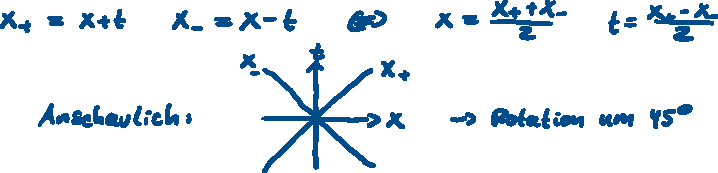
\includegraphics[width=.90\textwidth]{Dateien/Lichtkegel.pdf}
\end{center}
    Für die Funktion
    $$v(x_+, x_-)= u(\frac{x_++x_-}{2}, \frac{x_+-x_-}{2})$$
    lässt sich die Wellengleich in die Form
    $$v_{x_+x_-}=0$$
    bringen. Mit der Integration bekommen wir:
    $$v=w_1(x_+)+w_2(x_-) \Rightarrow u(x,t) = w_1(x+t)+w_2(x-t)$$
    Wobei $w_1$ und $w_2$ beliebig sind.
\end{Def}
\begin{Def}{Schwingende Saite}
    Für $u(x,t)$ gilt die Wellengleichung
    $$u_{xx}-u_{tt}=0$$
    Jeder Punkt kann eine Startauslenkung
    $$u_0(x)=u(x,0)$$
    und eine Anfangsgeschwindigkeit
    $$u_1(x)=u_t(x,0)$$
    haben. Diese nennt man \red{Anfangsbedingungen}. Für die Ränder $x=0$ und $x=1$ kann man unterschiedliche Randbedingungen wählen:
    \begin{enumerate}
        \item $u(0,t)=u(l,t)=0 \quad t\in [0,\infty)$, dies entspricht einer fest eingespannten Saite.
        \item $u_x(0,t)=u_x(l,t)=0 \quad t\in [0,\infty)$, dies entspricht einer freien Saite. Das sind die \red{von-Neumann-Randbedingungen}
        \item $u_t(0,t)=u_t(l,t)=0 \quad t\in(0,\infty)$, dies bedeutet, dass sich die Endpunkte nur mit konstanten Geschwindigkeit bewegen dürfen. Das sind die \red{Dirichlet-Randbedingungen}
    \end{enumerate}
\end{Def}
\begin{Def}{Unendlich lange Saite}
Für die unendlich lange Saite ist die Lösung durch die d'Alembert'sche Formel gegegen:
$$u(x,t)=\frac{1}{2}(u_0(x+t)+u_0(x-t)+\int_{x-t}^{x+t}u_1(\tau)d\tau)$$
Sie erfüllt die Anfangsbedingungen
$$u(x,0)=u_0(x)$$
$$u_t(x,0)=u_1(x)$$
\end{Def}
\begin{Def}{Endlich lange Saite mit dem Produktansatz}
    Sei $$u_{xx}-u_{tt}=0$$
    die Wellengleichung mit den Anfangsbedingungen
    $$u(x,0)=u_0(x)$$
    $$u_t(x,0)=u_1(x)$$
    mit den \blue{Dirichlet-Randbedingungen}:
    $$u_t(0,t)=u_t(\pi, t)=0$$
    Die Idee lautet, dass man dolgenden Produktansatz macht:
    $$u(x,t)=\alpha(x)\beta(t)$$
    Daraus folgt\footnote{Die Brüche sind Konstant}:
    $$u_{xx}(x,t)-u_{tt}(x,t)=\alpha''(x)\beta(t)-\alpha(x)\beta''(t)=0$$
    $$\iff \mu=\frac{\alpha''(x)}{\alpha(x)}=\frac{\beta''(t)}{\beta(t)} \quad \forall x,t$$
    Wir erhalten nun zwei lineare Differentialgleichungen:
    $$\alpha''(x)=\mu\alpha(x) \qquad \beta''(t)=\mu\beta(t)$$
    Hierfür verwendet man den Exponentialansatz aus MfP2:
    $$P(\lambda)=\lambda^2-\mu\lambda^0=\lambda^2-\mu$$
    Definiere nun $\mu=-\omega^2$, dann sind die Nullstellen:
    $$P(\lambda)=\lambda^2+\omega^2=(\lambda-i\omega)(\lambda+i\omega)=0)\iff \lambda_1= -i\omega \quad \lambda_2= i\omega$$
    Die Lösung DGL ist dann gegeben durch:
    $$\alpha_1(x)=Ae^{i\omega x}+Be^{-i\omega x}=A\sin(\omega x)+B\cos(\omega x)$$
    $$\beta(t)=C\sin(\omega t)+ B\cos(\omega t)$$
    \\ \\
    Nun schauen wir uns die Randbedingungen an:
    $$u_t(0,t)=u_t(\pi, t)=0$$
    Mit unserem Produktansatz wird daraus
    $$\alpha(0)\beta_t(t)=\alpha(\pi)\beta_t(t)=0$$
    $$\alpha(0)=A\cdot 0 + B\cdot 1 = B = 0$$
    $$\alpha(\pi)=A\sin(\omega \pi)+ B\cos(\omega \pi) = A\sin(\omega \pi)=0$$
    Die Lösungen für unser Anfangs-Randwertproblem lauten also:
    $$\alpha_n(x)=A_n\sin(nx)$$
    $$\beta_n(x)=c_n\sin(nt)+D_n\cos(nt)$$
    oder Allgemein:
    $$u(x,t)=\sum_{i=1}^n \alpha_n(x)\beta_n(t)=\sum_{i=1}^n (a_n\cos(nt)+b_n\sin(nt))\sin(nx)$$
\end{Def}
\begin{Def}{Endlich lange Saite mit der d'Alembertscher Formel}
Sei die Saite $2\pi$-periodisch:
$$u(x,0)=\alpha(x)\beta(0)=u_0(x) \Rightarrow u_0(0)=u_0(\pi)=0$$
$$u_t(x,0)=\alpha(x)\beta_t(0)=u_1(x) \Rightarrow u_1(0)=u_1(\pi)=0$$
Mit dem Fourieransatz erhalten wir:
$$u_0(x)=A_0+\sum_{i=1}^n (A_n\sin(nx)+A_n'\cos(nx))$$
Also haben wir:
$$u_0(x)=\sum_{i=1}^n A_n\sin(nx) \quad u_1(x)=\sum_{i=1}^n B_n\sin(nx)$$ mit Koeffizienten:
$$A_n=\frac{1}{\pi}\int_0^{2\pi}u_0(\tau)\sin(n\tau)d\tau \qquad B_n=\frac{1}{\pi}\int_0^{2\pi}u_1(\tau)\sin(n\tau)d\tau$$
Setzt man das in die d'Alembertsche Formel, so erhalten wir:
$$u(x,t)=\frac{1}{2}(u_0(x-t)+u_0(x+t)+\int_{x-t}^{x+t}u_1(\tau)d\tau)$$
$$=\frac{1}{2}\sum_{i=1}^n [A_n(\sin(n(x-t))+\sin(n(x+t))+\int_{x-t}^{x+t}B_n\sin(n\tau)d\tau]$$
$$=\sum_{i=1}^n [a_n\cos(nt)+b_n\sin(nt)]\sin(nx)$$
Also wie mit dem Produktansatz: 
    $$u(x,t)=\sum_{i=1}^n (a_n\cos(nt)+b_n\sin(nt))\sin(nx)$$
\end{Def}
\begin{Beispiel}{Lösen einer PDGL}
    Sei $u_{xx}-u_t=0$ mit der Anfangsbedingung $u(x,0)=e^{-2x}$. Wie lautet die Lösung? \\ \\
    Hier können wir den Produktansatz anwenden:
    $$u(x,t)=v(x)\cdot w(t)$$
    $$\Rightarrow \frac{\partial^2}{\partial x^2}v(x)w(t)-\frac{\partial}{\partial_t}v(x)w(t)=0$$
    $$\Rightarrow \frac{1}{v(x)}\frac{\partial^2}{\partial x^2}v(x)=\frac{1}{w(t)}\frac{\partial}{\partial t}w(t)=konst.$$
    Daraus folgen zwei separate DGls:
    \begin{enumerate}
        \item $\frac{1}{v(x)}\frac{\partial^2}{\partial x^2}v(x)=c$
        \item $\frac{1}{w(t)}\frac{\partial}{\partial t}w(t)=c$
    \end{enumerate}
    Zu 1)
    $$\frac{d^2}{dx^2}v(x)=cv(x) \quad \mbox{Ansatz: }v(x)=\lambda_2e^{ax}+\lambda_3e^{-ax}$$
    $$\Rightarrow a=\sqrt{c}$$
    $$\Rightarrow v(x)=\lambda_2 e^{\sqrt{C}x}+\lambda_3 e^{\sqrt{C}x}$$
    Zu 2)
    $$\frac{d}{dt}w(t)=cw(t)$$
    $$\Rightarrow \ln(w(t))=ct+a$$
    $$\Rightarrow w(t)=e^{ct}e^a=\lambda_1 e^{ct}$$
    Zusammengesetzt erhält man:
    $$u(x,0)=e^{-2x}=\lambda_1\lambda_2 e^{\sqrt{c}x}+\lambda_1\lambda_3e^{-\sqrt{c}x}=e^{-\sqrt{c}x} \quad c=4$$
    Die Lösung ist also:
    $$u(x,t)=e^{4t-2x}$$
\end{Beispiel}
\begin{Beispiel}{Rechnen mit dem Separationsansatz}
    Die $m$-dimensionale Wellengleichung ist gegeben durch $\triangle_m u = c^{-2}u_{tt}$, wobei $c\in \R/\{0\}$. Benutze den Separationsansatz von Bernoulli
    $$u(x,t)=e^{i\omega t}v(x) \quad (\omega\in \C)$$
    um daraus die Helmholtz-Gleichung $\triangle_m v(x)=-\lambda v(x)$ abzuleiten. Dabei ist $\lambda\in \C$. Von welchem Typ ist diese PDGL? \\ \\
    Wir betrachten $\triangle_m u=c^{-2}u_tt$. Einsetzten des Separationsansatzes gibt:
    $$\triangle_m u(x,t)=e^{i\omega t}\triangle_m v(x)$$
    $$c^{-2}u_{tt}(x,t)=v(x)c^{-2}\partial_t^2(e^{i\omega t})=-v(x)\frac{\omega^2}{c^2}e^{i\omega t}$$
    $$\Rightarrow \triangle_m v(x)=-\frac{\omega^2}{c^2}v(x)=-\lambda v(x)$$
    mit $\lambda=\frac{\omega^2}{c^2}$
    Dies ist eine PDGL vom elliptischen Typ.
\end{Beispiel}